\chapter{Material and Methods}
\section{Dataset}
Consider a collection of $m$ assay endpoints, denoted by $A = \{a_1, a_2, \dots, a_m\}$ and a set of $n$ compounds represented as $C = \{c_1, c_2, \dots, c_n\}$.
We introduce a \emph{presence matrix} $P \in {\{0, 1\}}^{m \times n}$. In this matrix, each row, indexed by $i$, corresponds to an individual assay endpoint $a_i$, and each column, indexed by $j$, signifies the presence (1) or absence (0) of a compound $c_j$ in the respective assay endpoints.
For a visual representation, refer to Figure~\ref{fig:presence_matrix_aeid_chid}, which illustrates the \emph{presence matrix} $P$ encompassing all assay endpoints and compounds available in the \textit{invitroDBv3.5} dataset. A compound is considered present in an assay endpoint if it has undergone testing, leading to the availability of a corresponding concentration-response series. The sparsity of matrix $P$ arises from the fact that not all compounds undergo testing across all assay endpoints.

\begin{figure}[h]  % Placement options: h (here), t (top), b (bottom), p (page)
    \centering
    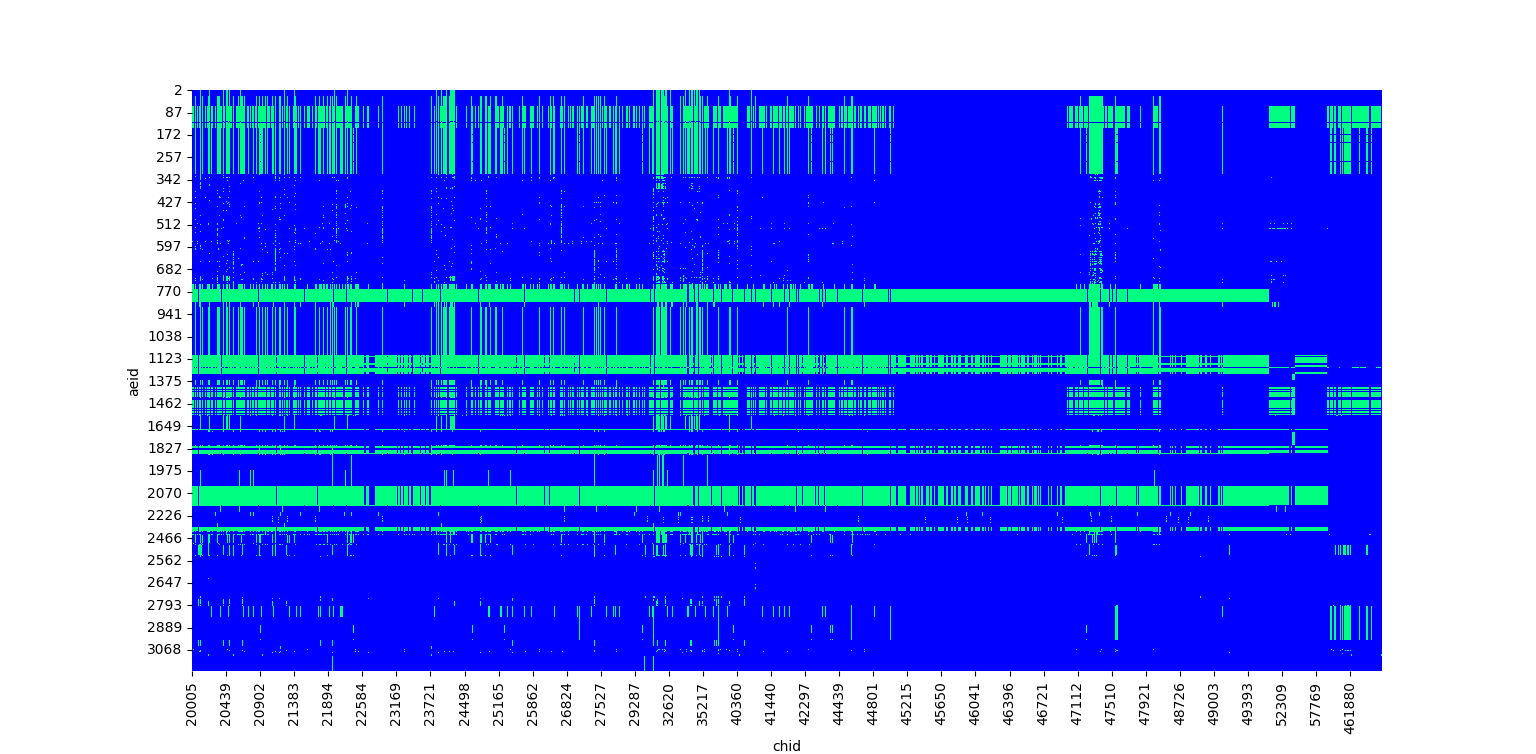
\includegraphics[width=0.7\textwidth]{figures/presence_matrix_aeid_chid.png}  
    \caption{The \emph{presence matrix} $P$ for $m = 271$ assay endpoints and $n = 9000$ compounds. The count, where $P_{ij} = 1$, indicates the availability of $3M$ concentration-response series for downstream analysis.}
~\label{fig:presence_matrix_aeid_chid} 
\end{figure}


A \textit{concentration-response series} is represented as a set of $k_{ij}$ concentration-response pairs: 
\[ S = \{(conc_1, resp_1), (conc_2, resp_2), \dots, (conc_k, resp_k)\} \]
where $conc_i$ values are not necessarily unique. 
In practice, concentrations are often subjected to multiple testing iterations, resulting in the formation of $n_{conc}$ distinct concentration groups. Within each concentration group, the number of replicates is indicated by $n_{rep}$.
Concentrations are transformed to the logarithmic scale using the unit $\mu M$ (micromolar), while the responses are normalized to either fold-induction or percent-of-control units.
Figure~\ref{fig:concentration_response_series} showcases a concentration-response series for a compound tested within a single assay endpoint.

\begin{figure}[htbp]  % Placement options: h (here), t (top), b (bottom), p (page)
    \centering
    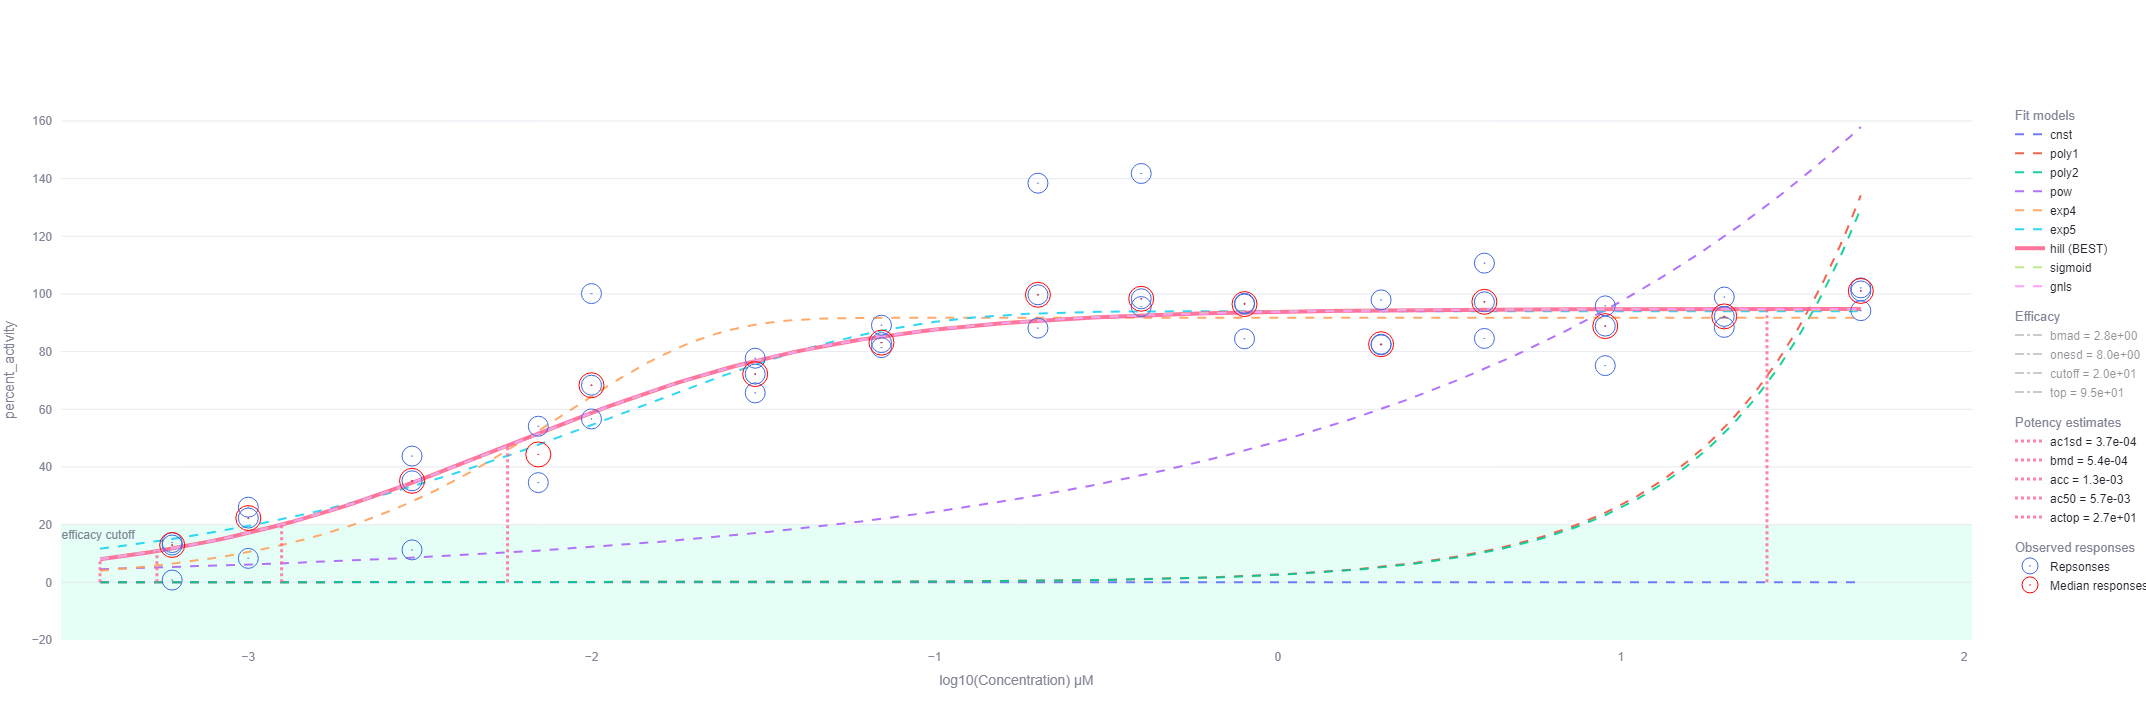
\includegraphics[width=1.0\textwidth]{figures/concentration_response_series_2.png}  
    \caption{A concentration-response series for the compound \textit{Estropipate} in the assay endpoint \textit{TOX21\_ERa\_LUC\_VM7\_Agonist}. The series has a total of $k = 45$ concentration-response pairs and is composed of $n_{conc} = 15$ concentration groups, each with $n_{rep} = 3$ replicates.}
~\label{fig:concentration_response_series} 
\end{figure}

\section{Pytcpl}
We introduce \href{https://github.com/rbBosshard/pytcpl}{pytcpl}, a streamlined Python package inspired by the R package \href{https://github.com/USEPA/CompTox-ToxCast-tcpl}{tcpl}, designed for processing high-throughput screening data. Our package is crafted to accomodate cusomizable processing steps and facilitate interactive data visualization with \href{https://pytcpl.streamlit.app/}{curve surfer} and empowers Python-oriented researchers to seamlessly engage in data analysis and exploration. It primarily focuses on providing essential features such as concentration-response curve fitting and allows for continuous hit-calling for compound bioactivity across diverse assay endpoints, akin to \href{https://github.com/USEPA/CompTox-ToxCast-tcplFit2}{tcplfit2}. Optionally, the \href{https://cfpub.epa.gov/si/si_public_record_Report.cfm?dirEntryId=355484&Lab=CCTE}{Invitrodb version 3.5 release} can serve as backend database if desired. The package optimizes data storage and compresses raw data and metadata from \emph{invitroDB} into Parquet files. This efficient strategy reduces storage needs, resulting in just 4 GB within the repository—compared to the original 80 GB database. This obviates the need for a cumbersome, large-scale database installation, rendering downstream analysis more accessible and efficient.

\section{Machine Learning Pipeline}
